\documentclass{article}
\usepackage{amsmath}
\usepackage{graphicx}
\usepackage{hyperref}
\begin{document}
\section{A source based experiment}\label{opening}

The imaginary laboratory records three samples without using personal records. Each sample has a readable description and a value in its original written form. The identifier 0012 names a series, while −7 records a signed change. The decimal point in 123.45 remains part of the observation. A revision can correct a transcription only while retaining the original document and a reason for the change.

$E=mc^{2}$

\section{Included observations}\label{observations}

The second observation separates content from its position on the page. A sentence can occupy two lines without changing its words, but a missing line changes the result. Empty cells are present in the table and do not ask the reader to invent a measurement. The figure contains colored regions, axes and a legend. A matching filename cannot establish that those elements survived conversion.

\[
\frac{x_i+1}{2}
\]

\[
\sum_{i=1}^{n}x_i
\]

\begin{table}
\begin{tabular}{lll}
Code & Value & Note\\
0012 & 0 & \\
B & −7 & 123.45
\end{tabular}
\caption{Measured cells}
\end{table}


\section{Structured results}\label{results}

\[
\begin{aligned}a&=1\\b&=-2\end{aligned}
\]

\[
\begin{bmatrix}0&-1\\2&3\end{bmatrix}
\]

\begin{figure}
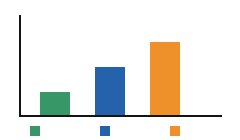
\includegraphics{assets/figure-en.png}
\caption{Figure 1 — Three regions and laboratory axes.}\label{fig1}
\end{figure}

See the figure and the source while keeping references explicit. \ref{fig1} \href{https://example.invalid/study?series=0012\&mode=a_b#note}{source} \cite{bib1}

\begin{thebibliography}{1}
\bibitem{bib1}Synthetic Researcher. Source notebook, 2026.
\end{thebibliography}


\end{document}
